\chapter{Situation-Awareness Applications}
\label{sec:apps}

\begin{comment}
- general
- specific exemplars in this dissertation
- application model
- functional requirements for implementing them
- platform services that would aid the functional realization of such apps
- Timing consideration for situation awareness apps
    * why cloud-based implementation falls short
    * motivate the need to move closer to the edge of the network
    * motivate the need for new mechanisms in geo-distributed edge
\end{comment}
The proliferation of high-fidelity sensors such as cameras, LiDAR, etc. and the increasing access to sophisticated data analysis and machine learning models has enabled the emergence of novel situation-awareness applications. These applications interact with the physical environment by sensing and extracting relevant information from it. Examples of such applications are collaborative sensing for autonomous driving - that fuses the data perceived by sensors on multiple cars to improve driving, collaborative pan-tilt-zoom tuning for a distributed camera network for tracking multiple targets simultaneously, etc. These applications form the target use-cases of this dissertation's research. This chapter discusses the characteristics of these applications and the underlying software platforms needed to support them \todo{something else?}.
\section{General Characteristics}
Situation-awareness applications possess common characteristics which are highlighted in the following.
\begin{itemize}
\item \textbf{Sense-process-actuate control loop. }  The applications of interest in this dissertation possess a sense-process-actuate control loop, wherein, applications sense the physical environment (e.g., through cameras or LiDAR sensors), extract information from the sensed data (e.g., the presence of a suspicious vehicle in a camera's view), and perform actions in response to events in the environment (e.g., moving the camera to better capture the target). This control loop functions at machine-perception speeds and does not involve human intervention in the critical path.
\item \textbf{Interaction with physical world in proximity. } Since the input data to target applications is sourced from sensors that measure the environment within their range, the application clients interact with events and objects (e.g., other clients) in their immediate physical vicinity. For example, autonomous cars are interested in objects in their immediate physical vicinity to make maneuvering decisions and avoid collisions. This property defines how application entities interact with one another.
\item \textbf{Inter-client collaboration}. Multiple clients of the same application, such as autonomous cars, are expected to be operating in the same physical space. Clients that are in proximity to each other (and hence interacting with an overlapping subset of the environment) benefit from sharing data among each other. Inter-client data sharing is necessary for the correct functionality of the application, such as in the case of collaborative PTZ tuning of cameras. It is also useful for improving each client's perception of the environment by augmenting the sensing range of each client and alleviating occlusion, such as in the collaborative sensing for autonomous driving application. 
\item \textbf{Client mobility.} Client devices in our target applications (e.g., drones, vehicles, etc.) are, by their very nature, mobile which leads to the environment that they are interacting with dynamic. Hence, the set of events that a client is interested in or the set of other clients that it collaborates with changes over time.
\item \textbf{Temporal variation in workload.} Given that the target applications sense the physical environment, the workload served depends on the amount of activity (e.g., number of cars in view of camera) in the sensing range of the client. However, in a typical environment (e.g., an urban area) the amount of activity varies temporally and spatially. Hence, both static and mobile clients would sense different levels of activity over time, and generate variable levels of workload.
\end{itemize}
\section{Specific Examples Used}
\subsection{Cooperative Sensing for Autonomous Driving}
Autonomous driving vehicles are reliant on local on-board sensors such as LiDAR and stereo cameras for detecting objects on and around the street such as a pedestrian crossing the street, etc. Unexpected events such as a jaywalking pedestrian or a vehicle jumping a red light warrant an immediate response in terms of braking or lane change. However, due to the inherent complexity of driving contexts in busy streets, it is possible that either the sensors are occluded by other objects in their field of view (\cref{fig:pedestrian}), or the sensing range of individual vehicles is not enough to capture the event (\cref{fig:redlight}) \cite{fusioneye}. To better cope with the above scenarios, the fusion of sensed data from multiple nearby vehicles along with road-side infrastructure (such as CCTV cameras) can alleviate the issues of limited sensing range and occlusion. For instance, as shown in \cref{fig:pedestrian} and \cref{fig:redlight}, the sensor data from nearby vehicles and CCTV cameras are used to augment the local sensors on-board each vehicle. This allows each vehicle to gain a wider view of the current traffic situation and become aware of the traffic event earlier.
\begin{figure*}[t!]
    \centering
    \begin{subfigure}[t]{0.45\textwidth}
        \centering
        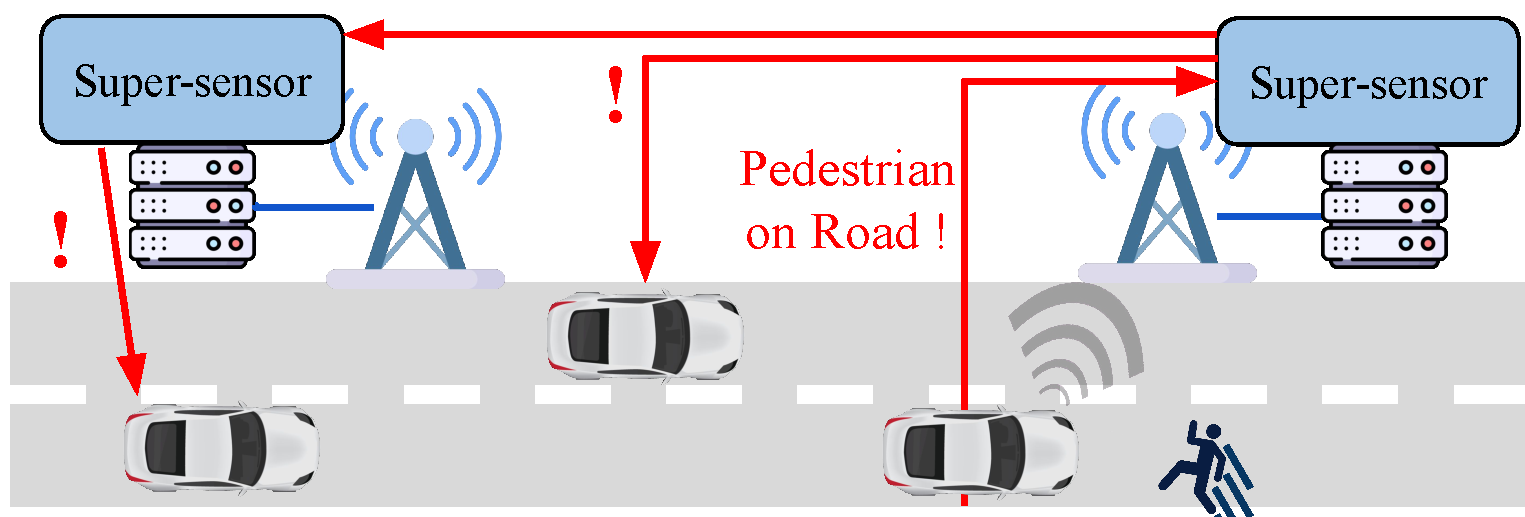
\includegraphics[width=\textwidth]{figures/apps/pedestrian}
        \caption{Detection of occluded pedestrians.}
        \label{fig:pedestrian}
    \end{subfigure}%
    ~ 
    \begin{subfigure}[t]{0.45\textwidth}
        \centering
        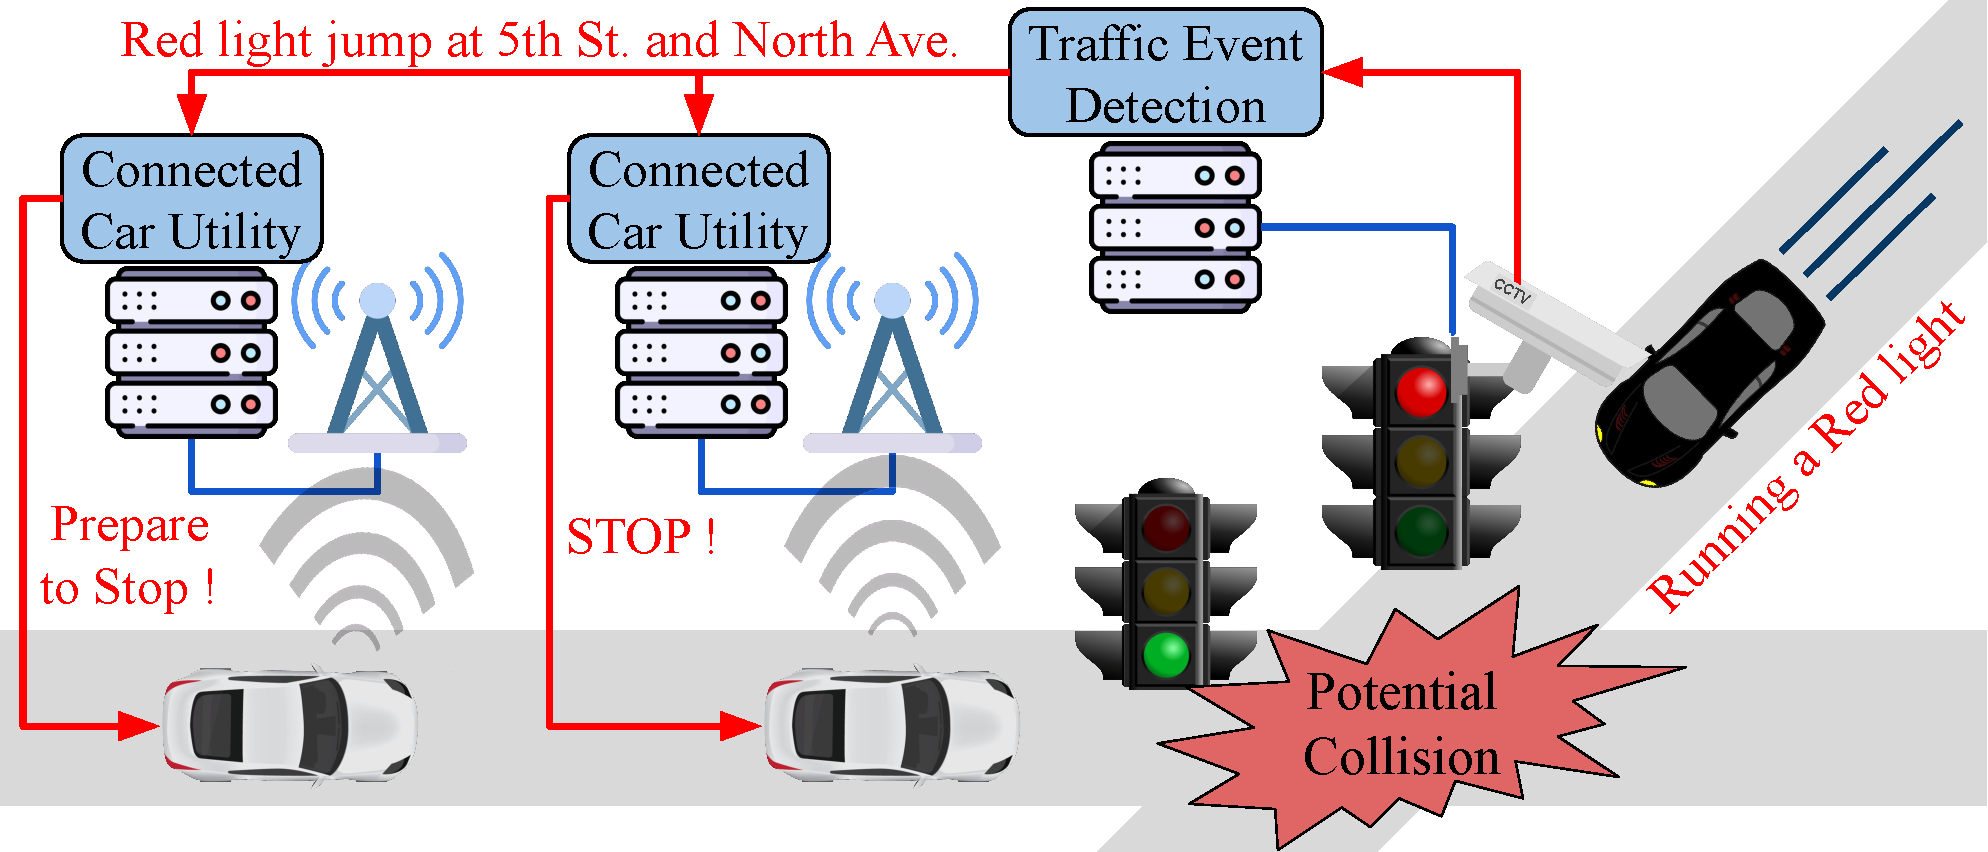
\includegraphics[width=\textwidth]{figures/apps/redlight}
        \caption{Notification of a rogue vehicle jumping a red light.}
        \label{fig:redlight}
    \end{subfigure}
    \caption{Use-cases of cooperative sensing for Autonomous driving.}
\end{figure*}
\par We assume the architecture of the cooperative driving application to be similar to that proposed by Boehme et al. \cite{talkycars}, which (to be best of the author's knowledge) is the only large-scale software architecture proposed for cooperative sensing. The application consists of a per-vehicle module that is responsible for pre-processing locally sensed data before fusion, and also merging the new information generated from fusion with the locally sensed information before sending it back to the vehicle. The fusion logic is handled by a number of Region Managers, each of which is responsible for handling the fusion of sensed data from vehicles in a particular geographical "region". The division of a geographical space (e.g., a city) into regions is done so as to ensure uniform load distribution across the Region Managers, however, that is out of the scope of this thesis.\footnote{Such a division can be done by taking into account historical levels of vehicular activity across space and ensuring that each region manager serves roughly uniform number of vehicles.}
\par The per-vehicle component for a given vehicle sends locally sensed data to the Region Manager corresponding to the vehicle's current location. Each vehicle has a logical area of interest (AoI) which represents the geographical area within which any information relevant to it is present. The AoI is typically centered on the vehicle's current location and changes dynamically as the vehicle moves. Each vehicle is interested in receiving the global view of road objects within its AoI, and hence reads fused sensor data from the Region Managers that overlap with its current AoI.

\subsection{Collaborative Navigation Control in UAV Swarm}
\begin{figure}[h]
\centering
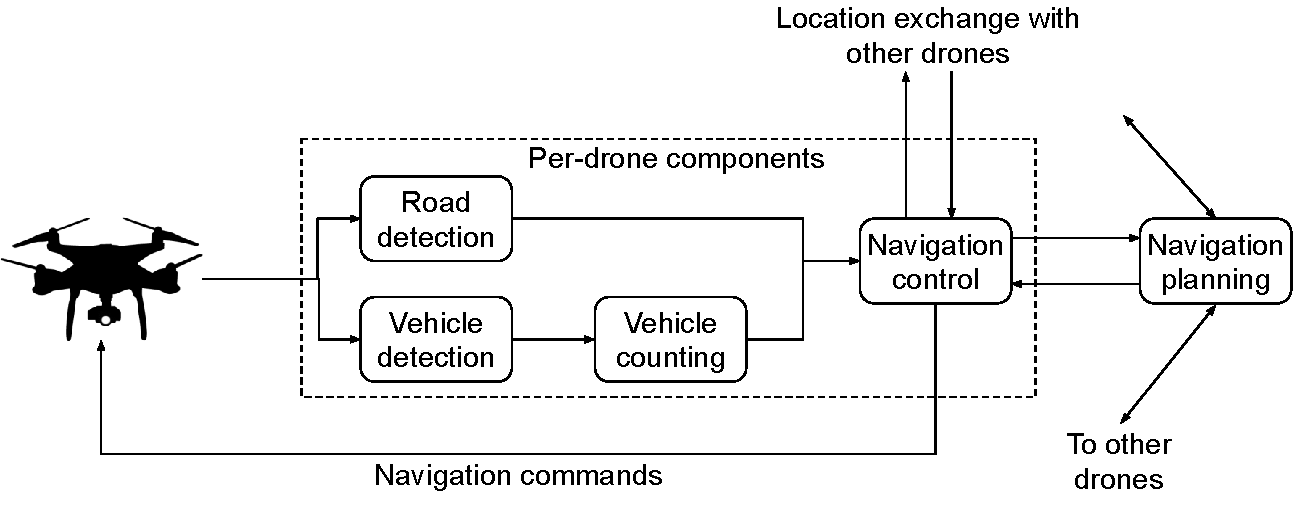
\includegraphics[width=0.75\columnwidth]{figures/apps/collab_drone_navigation}
\label{fig:collab_drone_navig}
\caption{Schematic of the Collaborative UAV Navigation application.}
\end{figure}

The limited range of cameras on an individual Unmanned Aerial Vehicle (UAV) makes it cumbersome to perform large-scale jobs such as traffic monitoring or search and rescue. However, given the low cost of UAVs and the availability of communication infrastructure, using a swarm of UAVs for this purpose makes the job much easier. Swarms of UAVs have been proposed to be used for road traffic monitoring \cite{huang2021decentralized}, search and rescue \cite{scherer2015autonomous} and surveillance \cite{meng2015skystitch}. Each UAV uses the local on-board sensors to extract information about objects in its field of view, such as the number of vehicles and their speeds. Each UAV shares this information with a control component, which computes the next action to be taken by each UAV, e.g., to monitor a given segment of the road. UAVs also communicate among each other for collision avoidance.

\subsection{Collaborative PTZ Tuning in a Distributed Camera Network}
Smart cities are seeing CCTV cameras installed at a large number of locations to record and analyze unexpected events such as accidents, crimes, etc. However, surveillance using CCTV cameras is largely done after an incident has occurred and the static deployment of cameras makes it difficult to fully capture the target objects. Contemporary cameras are often equipped with Pan-Tilt-Zoom tuning capabilities which allow them to better track target objects. Furthermore, due to the high density of cameras, they can also work collaboratively in tracking multiple target objects \cite{matsuyama2002real}.
\par In order to achieve this vision, the cooperative vision application groups cameras into multiple regions and splits the application logic between a per-camera component and a per-region Region Manager (see \cref{fig:multi_cam_ptz_app}). The per-camera processing component performs object detection and tracking and informs the region manager about the features of newly detected target objects and the current location of tracked target objects. It continuously tracks target objects by adjusting the PTZ parameters. The Region Manager consumes the current location of each target object and determines the assignment of camera to target object. In case a target object is about to leave the given region, the region manager informs the neighboring region(s) of the impending arrival of the target object.

\begin{figure}[h]
\centering
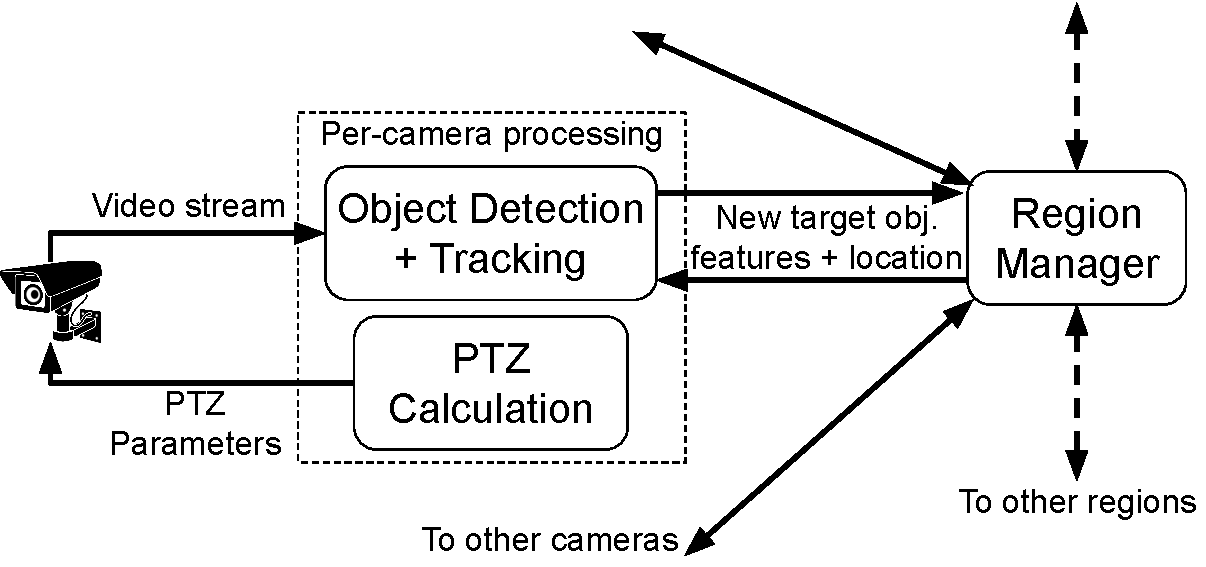
\includegraphics[width=0.75\columnwidth]{figures/apps/multi_cam_ptz}
\label{fig:multi_cam_ptz_app}
\caption{Schematic of Collaborative PTZ Tuning application for a Distributed Camera Network.}
\end{figure}

\section{Application Model}
\subsection{Computation}
\label{sec:app_model_compute}
The compute model of our target applications comprise of two main components.
\begin{itemize}
\item \textbf{Per-client component} for client-specific computation. This component is responsible for processing information generated by each client (e.g., an autonomous car or UAV) and providing input to higher layers of the application. The per-client component is specific to each application client and maintains the client's state.
\item \textbf{Region-level component} for combining information extracted from each client. Each region-level component is assigned a number of clients based on their geographical location. A given region-level component hosts  coordination and collaboration tasks between all the clients mapped to it. In the event that coordination between two clients belonging to two different regions is required, their two corresponding region-level components communicate between each other and share information.
\end{itemize}
%The compute requirements of the per-client component depends on the amount of activity perceived by the given client. Similarly, the compute requirements of a region-level component depends on the number of per-client components mapped to a it, and the workload generated by them. 
\subsection{Communication}
\label{sec:app_model_comm}
Communication among application entities in our target applications follow two primary patterns.
\begin{itemize}
\item Communication between the per-client component and region-level component. Clients share data with the corresponding region-level component for inter-client coordination and data-sharing within the region. Clients receive region-level information extracted from multiple clients. For example, in the collaborative PTZ tuning application, the per-camera component shares the current position of target objects currently assigned to it with the region manager, while receiving the locations of newly assigned target objects for it to track.
\item Area-of-Interest (AoI) based communication from a region-level component to per-client instances or other region-level components. A particular data-item is expected to be received by an application component if the data-item represents an object or event that falls within the receiver's AoI. This communication pattern can manifest itself in three ways: (1) region-level component to per-client component, as in the cooperative sensing application for autonomous driving, wherein a given vehicle receives the fused worldview not only from the region manager of the current region, but also from regions that overlap with the vehicle's area-of-interest. (2) across clients which fall in each other's AoI, as in the collaborative collision avoidance module of the UAV swarm application, which requires that UAVs share their current location among each other so that they can be aware of other UAVs in their vicinity. (3) communication between region-level components for sharing information at the region level. For instance, in the collaborative PTZ tuning application, region managers share details about a target object that is about to leave one region toward to other.
\end{itemize}
\subsection{Storage}
Applications generate state about application execution and information sensed from the environment, which needs to be persisted to enable future queries. Examples of such state include the assignment of target objects to PTZ cameras, semi-permanent road closures or traffic incidents in the collaborative driving application, etc. Such state if often tagged with the geo-location of the entity that it is describing, which is useful for executing range queries on geographical area. Data items in application's state are often read/updated by multiple entities. Applications expect a diverse set of  consistency guarantees on data access based on their application logic and reliance on most recent version of data.

\subsection{Spatial Affinity}
Since the target applications interact with the physical environment, actions taken by the application logic are often dependent on events and information from the immediate physical proximity. Hence, both computation and communication patterns of the target applications exhibit spatial affinity. Spatial affinity is defined by the Area-of-Interest of application clients and components, which represents the spatial area wherein other entities that the given entity directly interacts with are present. For instance, in the collaborative driving application, the area-of-interest of a car contains all other objects in vicinity of the car whose position information is needed in real-time to avoid potential collisions. Spatial affinity plays an important role in all facets of the application.
\begin{itemize}
\item \textbf{Computation. }Clients in physical proximity to each other are likely within each other's area-of-interest, and hence are grouped together and served by the same region-level application component. 
\item \textbf{Communication. } Communication patterns of the target applications is guided by spatial affinity of clients. Each client communicates with other clients and region-managers that fall within or overlap with the given client's area-of-interest. 
\item \textbf{Storage. }The state maintained and accessed by a application component pertains to objects and events in the subset of the physical environment that the application interacts with, and hence in physical proximity.
\end{itemize}

\section{Functional Requirements}
The target applications present a set of functional requirements on the underlying infrastructure. 
\begin{itemize}
\item \textbf{Low latency requirement. } The sense-process-actuate control loop of situation-awareness applications needs to be processed with end-to-end latency under the application's predefined threshold. This requirement ensures that the clients are able to respond in real-time to changes in the physical environment.
\item \textbf{Dynamic reconfiguration due to mobility. } Clients are continuously mobile, leading to changes in the network routes between the client devices and application components, which can result in a violation of the end-to-end latency threshold. Hence, the placement of application components needs to be adapted based on client's mobility to meet the latency requirements of the application. In addition to latency-driven reconfiguration, the mapping of per-client to region-level components needs to be reconfigured based on the current location of clients, so that inter-client coordination and data-sharing is done only between clients that are in geographical proximity of each other.
\item \textbf{Dynamic reconfiguration due to changing workload.} The workload experienced by application components (both per-client and region-level components) varies over time due to changing environmental conditions (e.g., changing number of cars detected by drones). This results in under- and over-utilization of allocated resources. Given the scarcity of edge resources and the need to continuously satisfy end-to-end latency requirements, the allocation needs to be updated so that performance requirements can be met without under-utilization of edge resources.
\end{itemize}
\section{Platform Services needed and Functional Requirements}
The aforementioned target applications can be implemented using a combination of platform services. Platform services provide the necessary systems support with powerful semantics for the applications, so that the developers can focus on the core application logic.

\subsection{Compute Orchestration}
The target applications comprise of multiple distributed components, each with a specific functionality. These application components require appropriate resource allocation to cater to their specific computational requirements such that a low sense-process-actuate control-loop latency can be ensured. Furthermore, for the application's correctness, per-client components should be mapped to the right region-level component based on client's current location. This problem is further complicated by the mobility of clients. Client mobility necessitates the dynamic reassignment of per-client components to region-level components because the set of clients present in a given region keeps changing over time. Furthermore, the spatial distribution of clients varies with time, and therefore the workload at each application component. This necessitates dynamic updates to the resource allocation of application components to avoid under-utilization or over-utilization of resources. 
\par Compute orchestration platform service handles all the above issues without requiring the developer's intervention. Given the latency and spatial affinity requirements of applications, the platform service will automatically deploy and reconfigure the resource allocation and connectivity of application components. Detecting the need for a reconfiguration entails continuously monitoring the processing latency of application components and mobility of clients respectively and checking if a violation of latency or spatial affinity occurred.

\begin{comment}
To ensure correct functionality of sense-process-actuate control loop, applications need to be deployed on edge sites to ensure that the end-to-end compute latency constraints imposed by the applications are satisfied. End-to-end latency refers to the total time taken to process a data item by all the application components from the time when it is generated by a client. End-to-end latency is not just a function of compute latency at each application component, but also the network latency between components - which in incurred to communicate the processing result of an upstream component to the downstream component. Hence, in addition to the amount of resources allocated to each application component on edge sites, the selection of the edge sites for hosting application components and network latencies between them  affects end-to-end latency. Furthermore, to serve the spatial affinity requirements of applications, per-client components need to be mapped to the right region-level component, so that data sharing can be done effectively. 
\par Clients are continuously mobile, which affects network latency between the client and the per-client application component, thereby affecting the end-to-end latency of the application. Moreover, mobile clients tend to frequently change the geographical regions that they belong to, which makes data sharing through their current region-level component ineffective. Hence, the placement of application components and the mapping of per-client component to region-level component needs to be dynamically updated to ensure continuous latency and spatial affinity satisfaction. Doing so also relies on monitoring the location of clients and experienced network latencies between clients and application components and detecting violations.
\par Dynamically managing application components of a large number of clients over a heterogeneous edge infrastructure is challenging for application developers. Hence, compute orchestration is a key platform service that reduces the burden of application developers by making sure that the application-specific requirements of latency and spatial affinity are satisfied. 
\end{comment}
\subsection{Publish-Subscribe Communication}
The communication patterns in the target situation-awareness applications ranges from one-to-many (region-level component to per-client component), many-to-one (per-client component to region-level component) and many-to-many patterns (among clients). Furthermore, given the continuous mobility of clients and the dependence of communication pattern on spatial affinity, the set of entities communicating with a given client changes over time. Implementing the communication subsystem for a given application would require maintaining a dynamically updated list of receivers for each data sender, ensuring reliable message delivery to all receivers, etc., which are challenging for application developers.
\par Publish-subscribe is a useful communication model, which uses the abstraction of "topics" to define interaction between entities. Special nodes called "brokers" host topics and perform message transfer from producers to consumers of each topic. The use of intermediary broker nodes allows the producers and consumers to be decoupled from each other. Data producers can send messages to a topic without waiting for it to be received by consumers, and consumers are notified asynchronously for each message. Publish-subscribe systems also maintain a persistent log of messages for each topic, which allows them to ensure strong data-delivery semantics, such as atleast-once delivery of messages to each consumer.

\subsection{Key-Value Storage}
The processing logic of our target applications depend on their state, hence it should be stored in a way that facilitates easy and efficient access. Key-value stores offer a convenient data model, wherein each data-item can be referenced using a unique key for reading and writing. Typically, key-value stores maintain multiple replicas of each data-item to ensure tolerance from failures. The network connectivity of data replicas and the number of replicas chosen for performing a read or write operation determines the operation latency and the consistency. Supporting a diverse set of applications with different latency and consistency guarantees requires that replica selection takes into account both the requirements of the application as well as the infrastructure topology.

\section{Timing considerations for situation-awareness applications}
\subsection{Why cloud-based solutions fall short?}
A number of platform services offering compute orchestration (e.g., Kubernetes), publish-subscribe communication (e.g., Apache Pulsar) and key-value storage (Apache Cassandra) are available for the cloud computing ecosystem. These services are widely used since they provide strong data-plane semantics (such as Cassandra's tunable consistency levels and Pulsar's at-least-once message delivery guarantee). In addition to useful semantics, the data-plane of these systems have been tuned for providing high throughput and low latency. 
\par However, relying on cloud-based solutions necessitates communicating with a remote datacenter location through the wide area network (WAN), and sending all of the data from client's sensors to the datacenter. Traversal through the WAN incurs high and unpredictable communication latency, and the large volume of high-fidelity sensor data (e.g., stereo cameras, LiDAR, etc.) causes high backhaul bandwidth consumption. 

\subsection{Need to move to the network edge}
Edge computing \cite{edge} presents a viable deployment alternative for the aforementioned platform services. The presence of computation and storage resources in proximity to the clients makes it possible reduce the network latency between the clients and application components. Edge infrastructure is a continuum of geo-distributed \emph{sites} hosted by multiple providers, such as telecommunication network providers, co-location providers (e.g., Vapor IO \cite{}), etc. An edge site typically comprises of a rack of server-grade machines, equipped with storage and networking infrastructure. Edge infrastructure has a wide geographical coverage in order to provide low-latency access to a large number of users. The wide geographical coverage coupled with heterogeneous connectivity results in non-trivial communication latencies between edge sites.  
\subsection{New mechanisms are needed at the edge}
The cloud-based platform services don't offer the same performance when deployed as-is on edge infrastructure because their control-plane policies are not optimized for an edge setting. These systems have been designed for operating in a datacenter setting, wherein machines are connected to each other via a high-throughput low-latency network. Clients, compute and data entities are co-located in the same datacenter, making the network latencies between these components negligible as compared to the compute and data access latencies. Hence, in these systems, the key to ensuring bounded end-to-end latency is uniform load balancing that prevents the formation of workload hotspots and therefore latency inflation. Using such systems as-is in an edge computing environment would result in the placement of compute and data entities on edge sites in a way that is agnostic of network latencies between edge sites - making the satisfaction of end-to-end latency requirements difficult. Furthermore, cloud-based platform services don't monitor observed end-to-end latencies to detect a violation and trigger reconfiguration.
\par In order to better serve the target applications, we need to introduce new edge-specific mechanisms into the control-plane of the platform services. Doing so will allow them to operate effectively in an edge setting and meet the requirements of applications.